\customchapter{Test and Debug}
\section{Scan Chain}

In VLSI design, a scan chain is a technique used for testing and debugging digital circuits. It is employed to facilitate the efficient testing of integrated circuits by enabling the observation and control of internal signals.
\vspace{2mm}

\begin{figure}[h] % Use the 'h' option to try to place the image "here"
  \centering
  \setlength{\abovecaptionskip}{-10pt} % Reduce space above the caption
  \setlength{\belowcaptionskip}{-10pt} % Adjust space below the caption
  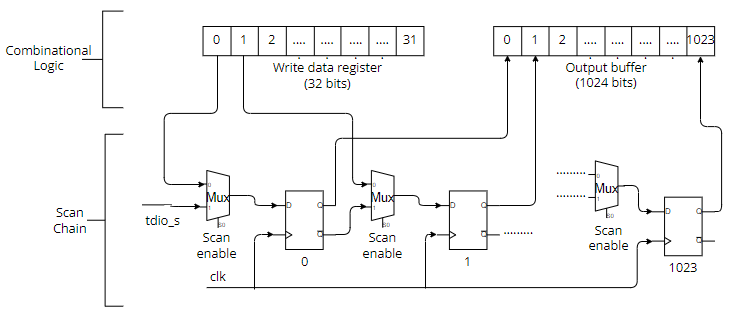
\includegraphics[width=0.9\textwidth]{Image/scan chain.png} % Replace 'your-image.png' with the actual file name
  \caption{Scan Chain Implementation}
  \label{Figure 1 : Scan Chain Implementation}
\end{figure}
\vspace{2mm}
The basic idea behind a scan chain is to create a serial path that connects all the scan flip-flops in the design. This serial path forms a shift register that allows you to shift in test vectors and observe the corresponding outputs. This capability is particularly useful for performing scan-based testing, which involves serially scanning in test patterns and capturing the responses.


\vspace{2mm}
This scan chain is implemented in the register file to store the data sent from other peripherals into the register file. Since the register file is designed to have 32x 32bit- registers a scan chain of 1024 scan flip-flops has been designed in the register file as mentioned in section 5.1.4.
\vspace{5mm}
\section{Design}

In the context of a scan chain, each flip-flop is specifically designed with supplementary input and output features to streamline the scan testing process. These additional elements typically consist of a serial scan input (SI) and a scan output (SO).


\vspace{2mm}
The serial scan input, sourced from the TDI port of the TAP controller, facilitates the introduction of test data into the flip-flop, where it is subsequently shifted into the following flip-flops. Another input for the scan flip-flop is the parallel data input, which originates from the internal register (WD3) of the register file.


\vspace{2mm}
The scan flip-flop is capable of storing data from either of these input sources at any given moment. To achieve this capability, a multiplexer (mux) is integrated into the input port of the scan flip-flop. The control of this mux is governed by a scan enable signal, determining which data is to be stored in the scan flip-flop.


\vspace{2mm}
Illustrated in the accompanying figure 7.1, each scan flip-flop features two output ports, both yielding identical output data – the information stored in the flip-flop. One output port is linked to the output buffer of the register file, while the other connects to the serial data input port of the subsequent flip-flop. This configuration establishes a scan chain, enabling diverse tests to be conducted on the designed hardware.


\vspace{2mm}

\section{Operation}

The scan has two operating modes as mentioned below:

\begin{itemize}
    \item \textbf{Normal mode: }In regular operation, the scan chain remains inactive, and the flip-flops function conventionally, operating as part of a standard sequential circuit. The designated scan flip-flops serve as registers within the register file, capturing parallel data from the 32-bit WD3 internal register of the register file. WD3 holds data intended for writing into the register file. The design of the scan flip-flops ensures that the data from the WD3 register is stored sequentially in the corresponding 32 scan chain flip-flops based on the 5-bit address stored in the A3 internal register of the register file.


    Subsequently, the data stored in the scan flip-flops is written into a 1024-bit wide output buffer during the falling edge of the clock cycle. In read operations of the register file, the data from the output buffer is transferred to the RD1 and RD2 internal 32-bit registers of the register file, contingent on the addresses present in the A1 and A2 ports. All these operation happen when the scan enable signal is low and allows parallel data to be stored into the scan flipflops.
    
\end{itemize}



\begin{itemize}
    \item \textbf{Scan mode: }This mode activates when the scan enable signal is set high, permitting the storage of data from the tdio\_s signal into the initial scan flip-flop. In this state, data is sequentially shifted into the scan flip-flops via the TDI port of the TAP controller.


    Upon each rising clock edge, data undergoes a rightward shift from one scan flip-flop to the next. Conversely, during the falling edge of each clock cycle, the data existing in the scan flip-flops becomes accessible at the scan input port of the succeeding flip-flop. Consequently, with each clock cycle, data undergoes a right shift, and the information present in the 1024th flip-flop is shifted out into the TDO signal of the TAP controller.
    
\end{itemize}
    The use of scan chains makes it easier to apply test patterns and observe responses during the testing phase of semiconductor manufacturing. This helps identify faults and defects in the integrated circuit, contributing to improved quality and reliability of the final product. The scan chain is also valuable for debugging and analyzing the behavior of a circuit during development.
\pagebreak
\newpage








